\documentclass[german]{beamer}

\mode<presentation>
{
 \usetheme{Madrid}

% \usecolortheme{crane}
 \usecolortheme{wolverine}
}

\usepackage{hyperref}

\usepackage[german]{babel}
\usepackage{times}
\usepackage[latin1,utf8]{inputenc}
\usepackage[OT2,T1]{fontenc}
\usepackage{shuffle}


% Stefan's abbreveations
\newcommand{\bq}{\begin{eqnarray*}}
\newcommand{\eq}{\end{eqnarray*}}
\newcommand{\eps}{\varepsilon}

\definecolor{MyYellowOrange}{cmyk}{0,0.5,1,0}
\newcommand{\superalert}[1]{{\color{MyYellowOrange}{#1}}}
\newtheorem*{myemptytheorem}{}

% dedicated environments
\newtheorem*{mytheorem27}{Hauptsatz der Differential- und Integralrechnung:} 

%%%%%%%%%%%%%%%%%%%%%%%%%%%%%%%%%%%%%%%%%%%%%%%%%%%%%%%%%%%%%%%%%%%%%%%%%%%%%%%%%%%%%%%%%%%%%%%%%%%%%%%%%
%%%%%%%%%%%%%%%%%%%%%%%%%%%%%%%%%%%%%%%%%%%%%%%%%%%%%%%%%%%%%%%%%%%%%%%%%%%%%%%%%%%%%%%%%%%%%%%%%%%%%%%%%
%%%%%%%%%%%%%%%%%%%%%%%%%%%%%%%%%%%%%%%%%%%%%%%%%%%%%%%%%%%%%%%%%%%%%%%%%%%%%%%%%%%%%%%%%%%%%%%%%%%%%%%%%

\title{Funktionen mehrerer Variablen}

\subtitle{Mathematischer Br\"uckenkurs}

\author{Stefan Weinzierl}

\institute[Uni Mainz]{Institut f\"ur Physik, Universit\"at Mainz}%

\date[WiSe 2020/21]{Wintersemester 2020/21}

\begin{document}

%%%%%%%%%%%%%%%%%%%%%%%%%%%%%%%%%%%%%%%%%%%%%%%%%%%%%%%%%%%%%%%%%%%%%%%%%%%%%%%%%%%%%%%%%%%%%%%%%%%%%%%%%
%%%%%%%%%%%%%%%%%%%%%%%%%%%%%%%%%%%%%%%%%%%%%%%%%%%%%%%%%%%%%%%%%%%%%%%%%%%%%%%%%%%%%%%%%%%%%%%%%%%%%%%%%
%%%%%%%%%%%%%%%%%%%%%%%%%%%%%%%%%%%%%%%%%%%%%%%%%%%%%%%%%%%%%%%%%%%%%%%%%%%%%%%%%%%%%%%%%%%%%%%%%%%%%%%%%

\begin{frame}
  \titlepage
\end{frame}

%%%%%%%%%%%%%%%%%%%%%%%%%%%%%%%%%%%%%%%%%%%%%%%%%%%%%%%%%%%%%%%%%%%%%%%%%%%%%%%%%%%%%%%%%%%%%%%%%%%%%%%%%
%%%%%%%%%%%%%%%%%%%%%%%%%%%%%%%%%%%%%%%%%%%%%%%%%%%%%%%%%%%%%%%%%%%%%%%%%%%%%%%%%%%%%%%%%%%%%%%%%%%%%%%%%
%%%%%%%%%%%%%%%%%%%%%%%%%%%%%%%%%%%%%%%%%%%%%%%%%%%%%%%%%%%%%%%%%%%%%%%%%%%%%%%%%%%%%%%%%%%%%%%%%%%%%%%%%

\section{Partielle Ableitungen}

\frame{\sectionpage}

% page --------------------------------------------------------------------------------------------------
\begin{frame}{Funktionen mehrerer Variablen}

\begin{definition}
Sei $U$ eine Teilmenge des ${\mathbb R}^n$.
Wir betrachten Funktionen
\bq
 f & : & U \rightarrow {\mathbb R},
 \nonumber \\
 \left( x_1, ..., x_n \right) & \rightarrow & f\left(x_1,...,x_n\right).
\eq
\end{definition}

\begin{example}
$U = {\mathbb R}^2$.
\bq
 f\left(x_1,x_2\right)
 & = & x_1^2 + x_2^2
\eq
\end{example}

\end{frame}

% page --------------------------------------------------------------------------------------------------
\begin{frame}{Partielle Ableitung}

\begin{definition}
Die Funktion $f$ ist {\bf partiell differenzierbar in der $i$-ten Koordinate}, falls der Grenzwert
\bq
 \lim\limits_{h \rightarrow 0} \frac{f\left(x_1,...,x_i+h,...,x_n\right)-f\left(x_1,...,x_i,...,x_n\right)}{h}
\eq
existiert.
\end{definition}

Man schreibt
{\footnotesize
\bq
 \frac{\partial}{\partial x_i} f\left(x_1,...,x_i,...,x_n\right)
 & = &
 \lim\limits_{h \rightarrow 0} \frac{f\left(x_1,...,x_i+h,...,x_n\right)-f\left(x_1,...,x_i,...,x_n\right)}{h}.
\eq
}

Diese Formel zeigt auch, wie man die $i$-te partielle Ableitung berechnet: Man h\"alt alle anderen Variablen
$x_1$,...,$x_{i-1}$, $x_{i+1}$, ..., $x_n$ fest und nimmt die gew\"ohnliche Ableitung nach der Variablen $x_i$.

\end{frame}

% page --------------------------------------------------------------------------------------------------
\begin{frame}{Partielle Differenzierbarkeit}

\begin{definition}
Wir nennen eine Funktion {\bf partiell differenzierbar}, falls sie in allen Variablen partiell differenzierbar ist.
\end{definition}

\begin{definition}
Ebenso nennen wir eine Funktion {\bf stetig partiell differenzierbar}, falls sie partiell differenzierbar ist und alle
Ableitungen stetig sind.
\end{definition}

\end{frame}

% page --------------------------------------------------------------------------------------------------
\begin{frame}{Partielle Ableitungen}

\begin{example}
Wir betrachten die Funktion
\bq
 f & : & {\mathbb R}^3 \rightarrow {\mathbb R},
 \nonumber \\
 & & (x_1,x_2,x_3) \rightarrow \sqrt{x_1^2+x_2^2+x_3^2}.
\eq
Es ist
\bq
 \frac{\partial}{\partial x_1} f(x_1,x_2,x_3) & = & \frac{x_1}{\sqrt{x_1^2+x_2^2+x_3^2}},
 \nonumber \\
 \frac{\partial}{\partial x_2} f(x_1,x_2,x_3) & = & \frac{x_2}{\sqrt{x_1^2+x_2^2+x_3^2}},
 \nonumber \\
 \frac{\partial}{\partial x_3} f(x_1,x_2,x_3) & = & \frac{x_3}{\sqrt{x_1^2+x_2^2+x_3^2}}.
\eq
\end{example}

\end{frame}

% page --------------------------------------------------------------------------------------------------
\begin{frame}{Quiz}

\bq
 f\left(x,t\right) & = & 
 A \sin\left(x-vt\right)
 \nonumber \\
 \frac{\partial}{\partial t} f\left(x,t\right)
 & = & ?
\eq
\begin{description}
\item{(A)} \;\;\;\;\;\;$A \cos(x-vt)$
\item{(B)} \;\;\;$-A \cos(x-vt)$
\item{(C)} \;\;\;\;\;\;$v A \cos(x-vt)$
\item{(D)} \;\;\;$- v A \cos(x-vt)$
\end{description}

\end{frame}

% page --------------------------------------------------------------------------------------------------
\begin{frame}{H\"ohere partielle Ableitungen}

\begin{definition}
Wir k\"onnen partielle Ableitungen auch hintereinander ausf\"uhren und erhalten h\"ohere Ableitungen:
\bq
 \frac{\partial}{\partial x_i} \frac{\partial}{\partial x_j} f\left(x_1,...,x_n\right)
 & = & 
 \frac{\partial}{\partial x_i} \left( \frac{\partial}{\partial x_j} f\left(x_1,...,x_n\right) \right).
\eq
\end{definition}

Man beachte, da{\ss} diese Schreibweise impliziert, da{\ss} zun\"achst die Ableitung nach $x_j$
ausgef\"uhrt wird, und das Zwischenergebniss dann nach $x_i$ abgeleitet wird.

\vspace*{4mm}
Wir interessieren uns daf\"ur unter welchen Voraussetzungen das Endergebniss nicht von der
Reihenfolge der Ableitungen abh\"angt.

\end{frame}

% page --------------------------------------------------------------------------------------------------
\begin{frame}{H\"ohere partielle Ableitungen}

\begin{theorem}
Satz: Sei $f$ zweimal stetig partiell differenzierbar. Dann gilt f\"ur die partiellen Ableitungen
\bq
 \frac{\partial}{\partial x_i} \frac{\partial}{\partial x_j} f\left(x_1,...,x_n\right)
 & = & 
 \frac{\partial}{\partial x_j} \frac{\partial}{\partial x_i} f\left(x_1,...,x_n\right)
\eq
\end{theorem}

\begin{theorem}
Allgemeiner gilt: Ist $f$ $k$-mal stetig partiell differenzierbar, so vertauschen die $k$-ten
partiellen Ableitungen:
\bq
 \frac{\partial}{\partial x_{i_1}} ... \frac{\partial}{\partial x_{i_k}} f\left(x_1,...,x_n\right)
 & = &
 \frac{\partial}{\partial x_{\sigma(i_1)}} ... \frac{\partial}{\partial x_{\sigma(i_k)}} f\left(x_1,...,x_n\right),
\eq
wobei $\sigma$ eine Permutation von $(i_1,...,i_k)$ ist.
\end{theorem}

\end{frame}

% page --------------------------------------------------------------------------------------------------
\begin{frame}{H\"ohere partielle Ableitungen}

\begin{example}
Wir betrachten die Funktion
\bq
 f & : & {\mathbb R}^3 \rightarrow {\mathbb R},
 \nonumber \\
 & & (x_1,x_2,x_3) \rightarrow x_1^3 + 3 x_1 x_2^2 + x_1 x_2 x_3
\eq
Es ist
\bq
 \frac{\partial}{\partial x_1} \frac{\partial}{\partial x_2} f(x_1,x_2,x_3) 
 & = & 
 \frac{\partial}{\partial x_1} \left( 6 x_1 x_2 + x_1 x_3 \right)
 \; = \; 6 x_2 + x_3
 \nonumber \\
 \frac{\partial^2}{\partial x_1^2} f(x_1,x_2,x_3) 
 & = & 
 \frac{\partial}{\partial x_1} \left( 3 x_1^2 + 3 x_2^2 + x_2 x_3 \right)
 \; = \; 6 x_1.
\eq
\end{example}

\end{frame}

% page --------------------------------------------------------------------------------------------------
\begin{frame}{Quiz}

\bq
 f\left(x_1,x_2\right) & = & 3 x_1^2 x_2^3
 \nonumber \\
 \frac{\partial}{\partial x_1} \frac{\partial}{\partial x_2} f\left(x_1,x_2\right)
 & = & ?
\eq
\begin{description}
\item{(A)} $0$
\item{(B)} $9 x_1^2$
\item{(C)} $18 x_1 x_2^2$
\item{(D)} $9 x_1^2 x_2^2 + 6 x_1 x_2^3$
\end{description}

\end{frame}

%%%%%%%%%%%%%%%%%%%%%%%%%%%%%%%%%%%%%%%%%%%%%%%%%%%%%%%%%%%%%%%%%%%%%%%%%%%%%%%%%%%%%%%%%%%%%%%%%%%%%%%%%
%%%%%%%%%%%%%%%%%%%%%%%%%%%%%%%%%%%%%%%%%%%%%%%%%%%%%%%%%%%%%%%%%%%%%%%%%%%%%%%%%%%%%%%%%%%%%%%%%%%%%%%%%
%%%%%%%%%%%%%%%%%%%%%%%%%%%%%%%%%%%%%%%%%%%%%%%%%%%%%%%%%%%%%%%%%%%%%%%%%%%%%%%%%%%%%%%%%%%%%%%%%%%%%%%%%

\section{Lokale Extremwerte}

\frame{\sectionpage}

% page --------------------------------------------------------------------------------------------------
\begin{frame}{Lokale Maxima und Minima}

\begin{definition}
Sei $f : {\mathbb R}^n \rightarrow {\mathbb R}$ eine zweimal stetig partiell differenzierbare Funktion.
Wir sagen, da{\ss} $f$ in $\vec{x}_0 \in {\mathbb R}^n$ ein {\bf lokales Maximum} hat, falls eine
Umgebung $U \subset {\mathbb R}^n$ von $\vec{x}_0$ existiert, so da{\ss}
\bq
 f\left(\vec{x}_0\right) & \ge & f\left(\vec{x}\right),
\eq
f\"ur alle $\vec{x}\in U$.
\end{definition}

\begin{definition}
Gilt dagegen
\bq
 f\left(\vec{x}_0\right) & \le & f\left(\vec{x}\right),
\eq
f\"ur alle $\vec{x}\in U$, so spricht man von einem {\bf lokalen Minimum}.
\end{definition}

\end{frame}

% page --------------------------------------------------------------------------------------------------
\begin{frame}{Lokale Maxima und Minima}

Eine \alert{notwendige Bedingung} f\"ur das Vorliegen
eines lokalen Minimums oder lokalen Maximums ist das \superalert{Verschwinden aller partiellen Ableitungen 
an der Stelle $\vec{x}_0$}:
\bq
 \left. \frac{\partial}{\partial x_i} f\left(\vec{x}\right) \right|_{\vec{x}=\vec{x}_0}& = & 0.
\eq
W\"urde eine partielle Ableitung nicht verschwinden, so gibt es in jeder Umgebung von $\vec{x}_0$ einen
Punkt, an dem $f(\vec{x})<f(\vec{x}_0)$ gilt, sowie einen Punkt an dem $f(\vec{x})>f(\vec{x}_0)$
gilt. Ist zum Beispiel die $i$-te partielle Ableitung ungleich Null, so betrachtet man hierzu
zwei Punkte, die um einen infinitessimalen positiven bzw. negativen Wert in Richtung des $i$-ten
Einheitsvektors verschoben sind.

\end{frame}

% page --------------------------------------------------------------------------------------------------
\begin{frame}{Die Hessesche Matrix}

Um eine hinreichende Bedingung f\"ur das Vorliegen eines lokalen Minimums oder Maximums zu finden
betrachten wir die zweiten Ableitungen und definieren die
{\bf Hessesche Matrix}:
\begin{definition}
\bq
 H_{ij}\left(\vec{x}\right) & = & \frac{\partial^2}{\partial x_i \partial x_j} f\left(\vec{x}\right),
 \;\;\; 1 \le i,j \le n.
\eq
\end{definition}
Da nach Voraussetzung $f$ zweimal stetig differenzierbar ist, vertauschen die partiellen Ableitungen
und die Hessesche Matrix ist offensichtliche symmetrisch:
\bq
 H_{ij}\left(\vec{x}\right) & = & H_{ji}\left(\vec{x}\right).
\eq

\end{frame}

% page --------------------------------------------------------------------------------------------------
\begin{frame}{Positiv definit, negativ definit und indefinit}

\begin{definition}
Wir bezeichnen eine symmetrische $n \times n$ Matrix $A$ als {\bf positiv definit}, falls
f\"ur alle $\vec{\xi} \in {\mathbb R}^n \backslash \{\vec{0}\}$ gilt:
\bq
 \vec{\xi}\,{}^T A \, \vec{\xi} & > & 0.
\eq
\end{definition}

\begin{definition}
Wir bezeichnen sie als {\bf negativ definit}, falls
f\"ur alle $\vec{\xi} \in {\mathbb R}^n \backslash \{\vec{0}\}$ gilt:
\bq
 \vec{\xi}\,{}^T A \, \vec{\xi} & < & 0.
\eq
\end{definition}

\begin{definition}
Wir bezeichnen die Matrix $A$ als {\bf indefinit}, falls es ein $\vec{\xi} \in {\mathbb R}^n$
und ein $\vec{\eta} \in {\mathbb R}^n$ gibt, so da{\ss}
\bq
 \vec{\xi}\,{}^T A \, \vec{\xi} > 0,
 & &
 \vec{\eta}\,{}^T A \, \vec{\eta} < 0.
\eq
\end{definition}

\end{frame}

% page --------------------------------------------------------------------------------------------------
\begin{frame}{Positiv semi-definit und negativ semi-definit}

Man findet auch die Begriffe ``positiv semi-definit'' und ``negativ semi-definit''. 

\begin{definition}
Eine symmetrische $n\times n$ Matrix $A$ nennt man {\bf positiv semi-definit} bzw.
{\bf negativ semi-definit}, falls f\"ur alle $\vec{\xi} \in {\mathbb R}^n$ gilt:
\bq
 \vec{\xi}\,{}^T A \, \vec{\xi} \ge 0,
 & \mbox{bzw.} &
 \vec{\xi}\,{}^T A \, \vec{\xi} \le 0.
\eq
\end{definition}

\end{frame}

% page --------------------------------------------------------------------------------------------------
\begin{frame}{Hurwitz-Kriterium}

Um zu entscheiden, ob eine symmetrische Matrix positiv definit ist, kann das Hurwitz-Kriterium
verwendet werden:

\begin{theorem}[Hurwitz]
Sei
\bq
 A & = & \left( \begin{array}{ccc}
 a_{11} & ... & a_{1n} \\
 ... & & ... \\
 a_{n1} & ... & a_{nn} \\
 \end{array} \right)
\eq
eine reelle symmetrische $n \times n$ Matrix.
$A$ ist positive definit, falls
\bq
 \left| \begin{array}{ccc}
 a_{11} & ... & a_{1k} \\
 ... & & ... \\
 a_{k1} & ... & a_{kk} \\
 \end{array} \right|
 & > & 0
\eq
f\"ur alle $k \in \{1,...,n\}$ gilt.
\end{theorem}

\end{frame}

% page --------------------------------------------------------------------------------------------------
\begin{frame}{Hurwitz-Kriterium}

\begin{example}
Die Matrix 
\bq
 A & = & \left( \begin{array}{ccc}
 3 & 1 & 1 \\
 1 & 4 & 1 \\
 1 & 1 & 5 \\
 \end{array} \right)
\eq
ist positiv definit:
\bq
 \left| \begin{array}{c}
 3 \\
 \end{array} \right|
 & = & 3,
 \nonumber \\
 \left| \begin{array}{cc}
 3 & 1 \\
 1 & 4 \\
 \end{array} \right|
 & = & 11,
 \nonumber \\
 \left| \begin{array}{ccc}
 3 & 1 & 1 \\
 1 & 4 & 1 \\
 1 & 1 & 5 \\
 \end{array} \right|
 & = & 50.
\eq
\end{example}

\end{frame}

% page --------------------------------------------------------------------------------------------------
\begin{frame}{Hurwitz-Kriterium}

\begin{theorem}
Eine reelle Diagonalmatrix
\bq
 A & = & \left( \begin{array}{cccc}
 \lambda_1 & 0 & ... & 0 \\
 0 & \lambda_2 & ... & 0 \\
 ... & & & ... \\
 0 & 0 & ... & \lambda_n \\
 \end{array} \right)
\eq
ist 
\begin{itemize}
\item positiv definit, falls alle Diagonaleintr\"age positiv sind:
\bq
 \lambda_j & > & 0,
 \;\;\;\;\;\; \forall \; 1 \le j \le n.
\eq
\item negativ definit, falls alle Diagonaleintr\"age negativ sind:
\bq
 \lambda_j & < & 0,
 \;\;\;\;\;\; \forall \; 1 \le j \le n.
\eq
\end{itemize}
\end{theorem}

\end{frame}

% page --------------------------------------------------------------------------------------------------
\begin{frame}{Hurwitz-Kriterium}

\begin{example}
Die Diagonalmatrix
\bq
 \left( \begin{array}{cccc}
 3 & 0 & 0 & 0 \\
 0 & 5 & 0 & 0 \\
 0 & 0 & 7 & 0 \\
 0 & 0 & 0 & 11 \\
 \end{array} \right)
\eq
ist positiv definit.
\end{example}

\end{frame}

% page --------------------------------------------------------------------------------------------------
\begin{frame}{Quiz}

Die Matrix
\bq
 \left( \begin{array}{rrrr}
 1 & 0 & 0 & 0 \\
 0 & -1 & 0 & 0 \\
 0 & 0 & 2 & 0 \\
 0 & 0 & 0 & -2 \\
 \end{array} \right)
\eq
ist 
\begin{description}
\item{(A)} positiv definit
\item{(B)} negativ definit
\item{(C)} negativ semi-definit
\item{(D)} indefinit
\end{description}

\end{frame}

% page --------------------------------------------------------------------------------------------------
\begin{frame}{Lokale Extremwerte}

Wir kehren zur Betrachtung der lokalen Minima und Maxima einer Funktion zur\"uck. Wir erhalten die
folgende Aussage:

\begin{theorem}
Sei $f : {\mathbb R}^n \rightarrow {\mathbb R}$ eine zweimal stetig partiell differenzierbare Funktion
und $\vec{x}_0\in {\mathbb R}^n$ ein Punkt, so da{\ss}
\bq
 \left. \frac{\partial}{\partial x_j} f(\vec{x}) \right|_{\vec{x}=\vec{x}_0} & = & 0,
 \;\;\; \forall 1 \le j \le n.
\eq
\begin{itemize}
\item Ist die Hessesche Matrix $H_{ij}(\vec{x}_0)$ positiv definit, so besitzt $f$ in $\vec{x}_0$
ein {\bf lokales Minimum}.
\item Ist sie negativ definit, so besitzt $f$ in $\vec{x}_0$ ein {\bf lokales Maximum}.
\item Ist die Hessesche Matrix indefinit, so sagt man, da{\ss} $f$ in $\vec{x}_0$ einen {\bf Sattelpunkt}
besitzt.
\end{itemize}
\end{theorem}

\end{frame}

% page --------------------------------------------------------------------------------------------------
\begin{frame}{Beispiel 1}

\begin{example}
Sei 
\bq
 f(x,y) & = & x^2 + y^2.
\eq
Im Punkte $\vec{x}_0=(0,0)$ verschwinden die partiellen Ableitungen:
{\footnotesize
\bq
 \left.\frac{\partial f}{\partial x}\right|_{\vec{x}=(0,0)}
 = \left. 2 x \right|_{\vec{x}=(0,0)}
 = 0,
 & &
 \left.\frac{\partial f}{\partial y}\right|_{\vec{x}=(0,0)}
 = \left. 2 y \right|_{\vec{x}=(0,0)}
 = 0.
\eq
}

\vspace*{-2mm}
Die Hessesche Matrix ist gegeben durch
{\footnotesize
\bq
 H(\vec{x}) & = & \left( \begin{array}{cc}
  2 & 0 \\
  0 & 2 \\
 \end{array} \right)
\eq
}

\vspace*{-2mm}
Diese Matrix ist positiv definit und $f$ hat an der Stelle $\vec{x}_0=(0,0)$ ein Minimum.
\end{example}

\end{frame}

% page --------------------------------------------------------------------------------------------------
\begin{frame}{Beispiel 1}

\begin{figure}
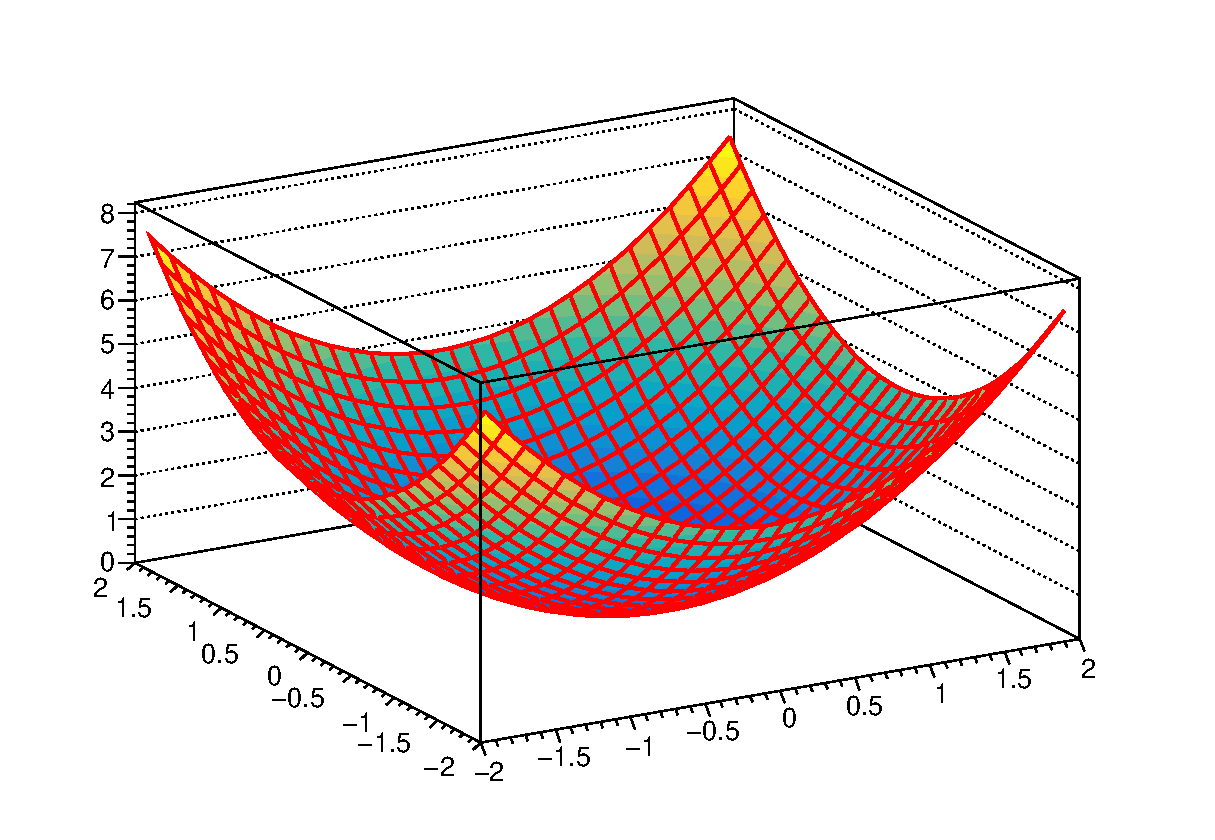
\includegraphics[scale=0.5]{minimum}
\end{figure}

\end{frame}

% page --------------------------------------------------------------------------------------------------
\begin{frame}{Beispiel 2}

\begin{example}
Sei nun
\bq
 f(x,y) & = & x^2 - y^2.
\eq
Im Punkte $\vec{x}_0=(0,0)$ verschwinden die partiellen Ableitungen:
{\footnotesize
\bq
 \left.\frac{\partial f}{\partial x}\right|_{\vec{x}=(0,0)}
 = \left. 2 x \right|_{\vec{x}=(0,0)}
 = 0,
 & &
 \left.\frac{\partial f}{\partial y}\right|_{\vec{x}=(0,0)}
 = \left. -2 y \right|_{\vec{x}=(0,0)}
 = 0.
\eq
}

\vspace*{-2mm}
Die Hessesche Matrix ist gegeben durch
{\footnotesize
\bq
 H(\vec{x}) & = & \left( \begin{array}{cc}
  2 & 0 \\
  0 & -2 \\
 \end{array} \right)
\eq
}

\vspace*{-2mm}
Diese Matrix ist indefinit und $f$ hat an der Stelle $\vec{x}_0=(0,0)$ einen Sattelpunkt.
\end{example}

\end{frame}

% page --------------------------------------------------------------------------------------------------
\begin{frame}{Beispiel 2}

\begin{figure}
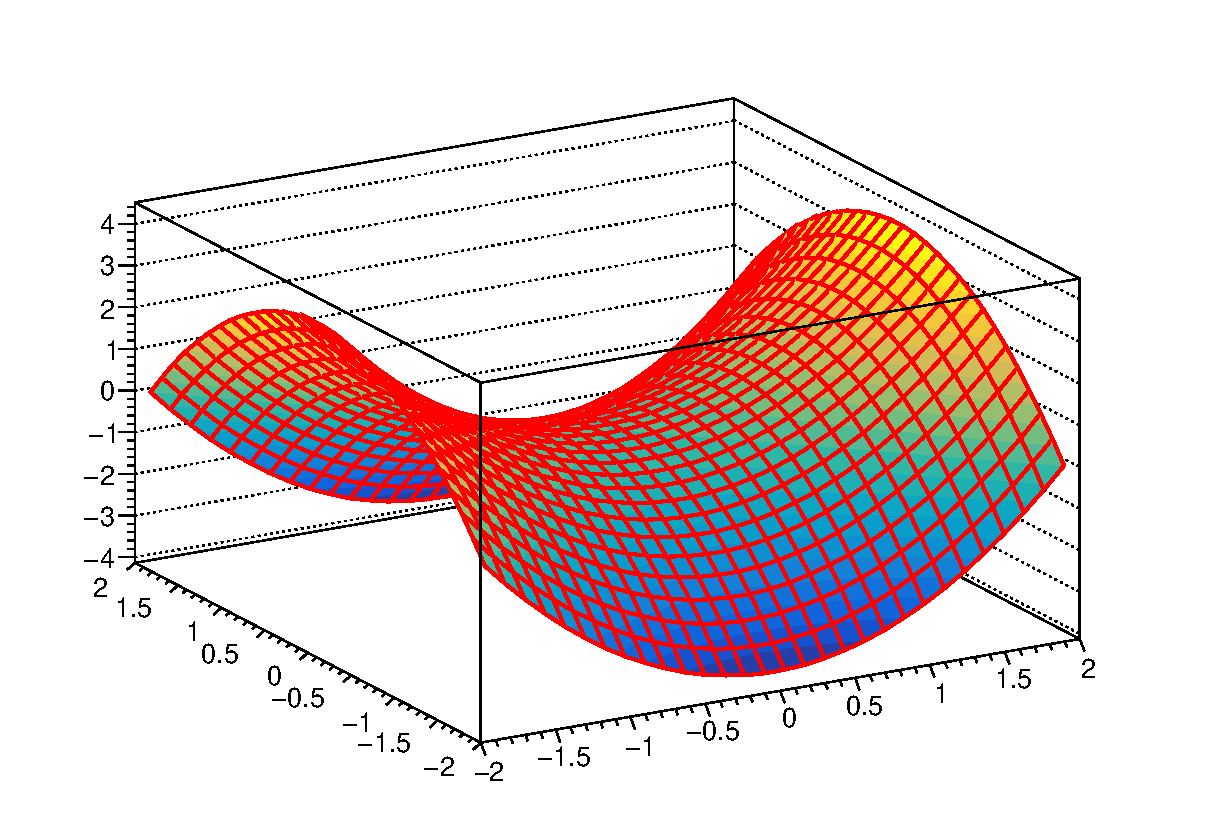
\includegraphics[scale=0.5]{saddlepoint}
\end{figure}

\end{frame}

%%%%%%%%%%%%%%%%%%%%%%%%%%%%%%%%%%%%%%%%%%%%%%%%%%%%%%%%%%%%%%%%%%%%%%%%%%%%%%%%%%%%%%%%%%%%%%%%%%%%%%%%%
%%%%%%%%%%%%%%%%%%%%%%%%%%%%%%%%%%%%%%%%%%%%%%%%%%%%%%%%%%%%%%%%%%%%%%%%%%%%%%%%%%%%%%%%%%%%%%%%%%%%%%%%%
%%%%%%%%%%%%%%%%%%%%%%%%%%%%%%%%%%%%%%%%%%%%%%%%%%%%%%%%%%%%%%%%%%%%%%%%%%%%%%%%%%%%%%%%%%%%%%%%%%%%%%%%%

% page --------------------------------------------------------------------------------------------------
\begin{frame}{Organisatorisches}

\begin{center}
\alert{Plenumsdiskussion heute um 13:00h}!
\end{center}

\end{frame}

% page --------------------------------------------------------------------------------------------------
\begin{frame}

\end{frame}

\end{document}


